\chapter{Design}

\section{Document management}

\subsection{The SharePoint library}

The Java implementation is split to two parts, the generic SharePoint library
and the user interface, which is an UNO component. The previous lives under the
\emph{hu.ulx.lpsp.sharepoint} namespace, the other does so under
\emph{hu.ulx.lpsp.comp}.

The UML package diagram on \autoref{fig:design-packages} diagram shows these
packages with their dependencies.

\begin{figure}[H]
\centering
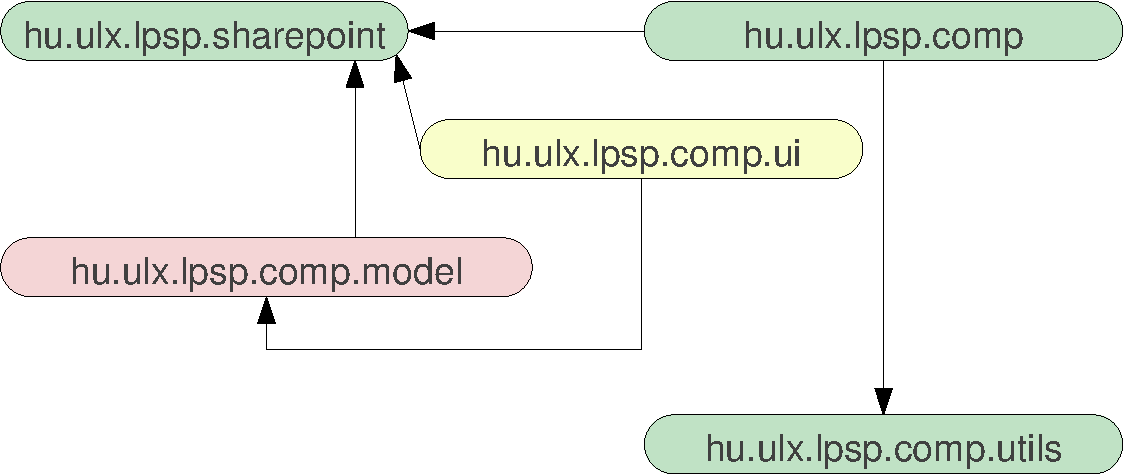
\includegraphics[width=425px,keepaspectratio]{design-packages.pdf}
\caption{Packages of the document management extension}
\label{fig:design-packages}
\end{figure}

At the time of writing, there is no ready to use Java library to communicate
with a SharePoint server. Because of this, we decided to separate the SharePoint
protocol implementation from the LibreOffice-specific part of the extension to
make it reusable in other projects. It provides the following classes:

\begin{itemize}
\item \emph{SPHandler}: Handles requests from a frontend. Unless a feature has a
specific class, it is implemented here.
\item \emph{FileOpenParser}: Parses the result from the \emph{list directory of
a workspace} request.
\item \emph{FileOpenRootParser}: Parses the result from the \emph{list
workspaces} request.
\item \emph{HandlerTest}: Automatically tests all features on a given server
using JUnit.
\item \emph{LastModParser}: Parses the result from the \emph{get last
modification date} request.
\item \emph{Messages}: Provides localization for the library error messages.
\item \emph{PacketParser}: Extracts the error message from a Vermeer
RPC \cite{vermeer} response packet.
\item \emph{Version}: Handles document versions.
\end{itemize}

We paid attention in our solution to not require additional server-side component
installation, the SharePoint library can communicate with a standard SharePoint
server, without any server modifications.

\subsection{The UNO interfaces}

\begin{figure}[H]
\centering
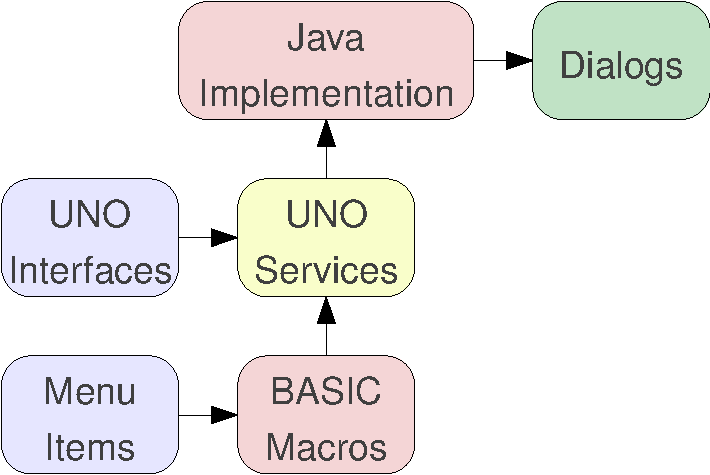
\includegraphics[width=400px,keepaspectratio]{design-technologies.pdf}
\caption{Technologies used in the design of the extension}
\label{fig:design-technologies}
\end{figure}

The UNO interfaces are inspired by the already referenced OPAL extension.
Where it made sense, we reused code from there, and changed it to work with
Sharepoint.

It's an UNO convention that interfaces start with a capital X. The following
\textbf{UNO interfaces} (see \autoref{fig:design-technologies}) are provided by the
extension:

\begin{itemize}
\item \emph{XSharepointFilePicker}: an open/save as file picker.
\item \emph{XSharepointVersions}: a versions dialog.
\item \emph{XAuthenticationManager}: a handler for different authentication mechanisms.
\item \emph{XConnection}: a connection to a SharePoint server.
\item \emph{XSharepointDocument}: a document received from the
SharePoint server.
\item \emph{XSharepointDocumentManager}: a storage for XSharepointDocument instances.
\end{itemize}

The extension provides a single exception type -- \emph{SharepointException} --
when it throws errors.

It also provides a single enumeration type -- \emph{FileTypes} -- to declare
the list of LibreOffice applications it handles. (It's current value is:
Writer, Calc, Impress and Draw.)

UNO services are interfaces containing static methods only.  The following
\textbf{UNO services} (see \autoref{fig:design-technologies}) are provided by the
extension:

\begin{itemize}
\item \emph{Connection}: implementation for XConnection.
\item \emph{SharepointDocument}: factory for XSharepointDocument.
\item \emph{theAuthenticationManager}: singleton for XAuthenticationManager.
\item \emph{theSharepointDocumentManager}: singleton for XSharepointDocumentManager.
\item \emph{SharepointFilePicker}: implementation for XSharepointFilePicker.
\item \emph{SharepointVersions}: implementation for XSharepointVersions.
\end{itemize}

\subsection{User interface}

The user interface lives in the \emph{hu.ulx.lpsp.comp} package. The classes of
the user interface are organized in 4 Java packages:

\begin{itemize}
\item \emph{hu.ulx.lpsp.comp.model}: a model for the folder and document
structure, used by the file pickers (\emph{open} and \emph{save as} dialog
windows).
\item \emph{hu.ulx.lpsp.comp.ui}: contains the dialog classes.
\item \emph{hu.ulx.lpsp.comp.util}: miscellaneous utility classes for UNO and localization.
\item \emph{hu.ulx.lpsp.comp}: classes implementing the rest of UNO
services: authentication manager, document manager, document, connection, etc.
\end{itemize}

The user interface dialogs are reachable from the \emph{Document repository}
menu item, which is registered by the \emph{Addons.xcu} configuration file,
which is a standard configuration file of LibreOffice extensions.

\subsubsection*{Menu items}

The following \textbf{menu items} (see \autoref{fig:design-technologies}) are designed:

\begin{itemize}
\item Connection: force connecting to an other document management server, even
if the user is already connected.
\item Open: downloads an existing document from the server.
\item Close: discards the local copy of a downloaded document.
\item Save: save the document model and upload the saved local copy to the server.
\item Save as: upload the local document to the server using a new name.
\item Versions: management of document versions.
\end{itemize}

The menu items call BASIC macros, which invoke UNO services. Those services are
finally implemented in the Java user interface.

\subsubsection*{Macros}

The macros are split into two packages: the ones directly called by the menu
items, and the other utility macros.

The menu items call the following \textbf{macros} (see
\autoref{fig:design-technologies}) in the \emph{LPSP.menu} package:

\begin{itemize}
\item openFile: shows the File Open dialog.
\item openVersion: shows the dialog listing versions of the document.
\item saveFile: saves the document via the document manager.
\item saveAsFile: shows the Save As dialog.
\item closeFile: closes the current document via the document manager, the
already registered close listener will handle the cleanup of the local document
copy.
\end{itemize}

The following ones are the utility macros (\emph{LPSP.utils} package):

\begin{itemize}
\item getCurrentSharepointDocument: asks the document model of the current LibreOffice component (Writer document, Calc spreadsheet, etc.) from the document manager.
\item getCurrentConnection: asks the current connection from the authentication manager.
\item getConnection: shows the Connection dialog.
\item getDocumentManager: returns the document manager singleton.
\item getAuthenticationManager: returns the document manager singleton.
\end{itemize}

The BASIC macros invoke the following UNO services:

\begin{itemize}
\item Connection: calls \emph{theAuthenticationManager::execute()}.
\item Open: calls \emph{SharepointFilePicker::execute()} with \emph{IsOpen = true}.
\item Close: calls \emph{theSharepointDocumentManager::getSharepointDocument()}, \\ then the \emph{close} method on the returned result.
\item Save: calls \emph{theSharepointDocumentManager::getSharepointDocument()}, \\ then the \emph{save} method on the returned result.
\item Save as: calls \emph{SharepointFilePicker::execute()} with \emph{IsOpen = false}.
\item Versions: calls \emph{SharepointVersions::execute()}
\end{itemize}

\subsubsection*{Java implementation}

At this point, we know the user interface entry points in our Java
implementation. As mentioned above, Java bytecode for the UNO services are
automatically generated (by \emph{javamaker}). The next task is to let the stub
know where is its implementation. This is handled by the
\emph{RegistrationHandler} class. The list of implementation classes
implementing a UNO service is in the \emph{RegistrationHandler.classes} file.
Each implementation class specifies what service does it implement, then the
registration handler collects this information and sends it to UNO, when it is
asked. Finally, the \emph{RegistrationClassName:} header in the
\emph{META-INF/MANIFEST.MF} file of the Jar package defines the registration
handler class name.

As a result, the following entry points are designed in the \textbf{Java
implementation} (see \autoref{fig:design-technologies}):

\begin{itemize}
\item Connection: \emph{AuthenticationManagerImpl.execute()}
\item Open: \emph{SharepointFilePickerImpl.execute()}
\item Close: \emph{SharepointDocumentManagerImpl.getSharepointDocument()}, \\ then \emph{SharepointDocumentImpl.close()}
\item Save: \emph{SharepointDocumentManagerImpl.getSharepointDocument()}, \\ then \emph{SharepointDocumentImpl.save()}
\item Save as: \emph{SharepointFilePickerImpl.execute()}
\item Versions: \emph{SharepointVersionsImpl.execute()}
\end{itemize}

These classes contain all the business logic and they call the SharePoint
library for communication. The dialog windows are separated from UNO
interfaces, they are always implemented in separate classes. Given that there
are common tasks for all of our user interface dialogs, there is a common
ancestor for all of them, called \emph{AbstractDialog}.

\subsubsection*{Dialog classes}

The following \textbf{dialog classes} (see \autoref{fig:design-technologies}) are included in the \emph{ui} package:

\begin{itemize}
\item Connection: \emph{ConnectionDialog} (connect dialog), \\
\emph{ConfigServerDialog} (server list), \\ \emph{ServerDialog} (settings for an
individual target)
\item Open, save as: \emph{FilePickerDialog}
\item Close: None.
\item Save: \emph{CommentVersionDialog}
\item Versions: \emph{VersionsDialog}
\end{itemize}

For an UML class diagram showing these classes, see \autoref{fig:design-spui}.

\begin{figure}[p]
\centering
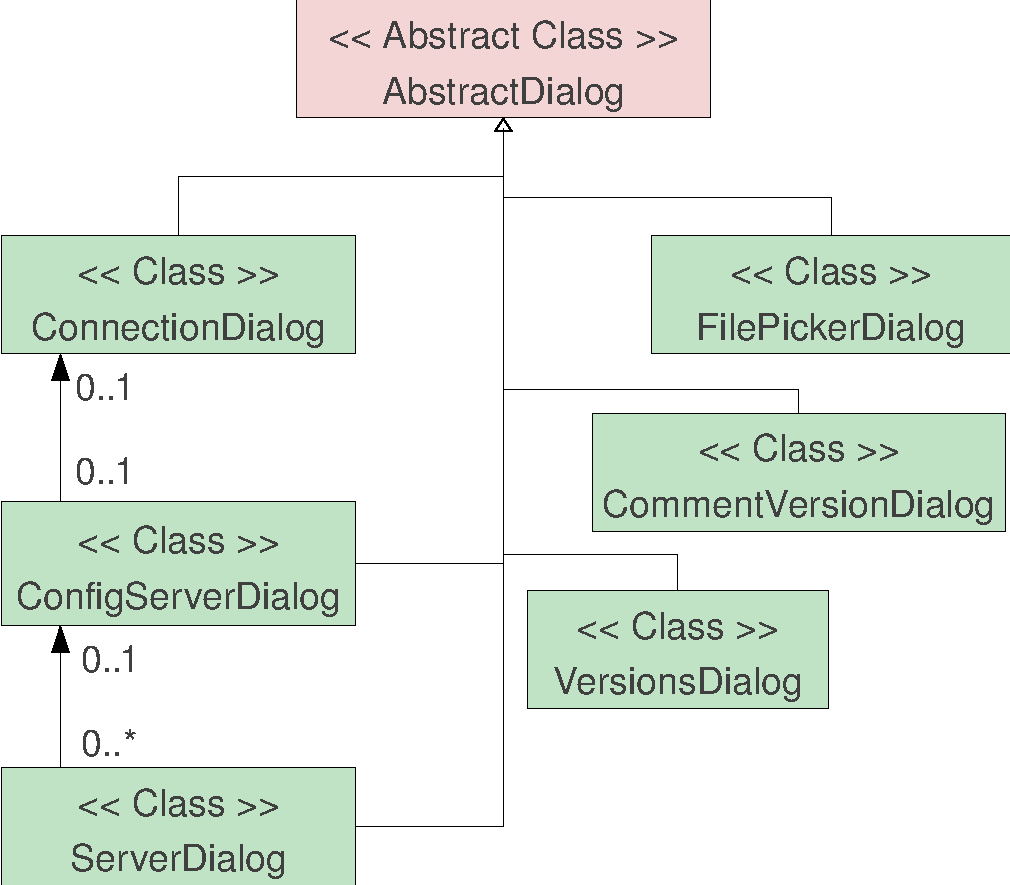
\includegraphics[width=400px,keepaspectratio]{design-spui.pdf}
\caption{Classes of the user interface}
\label{fig:design-spui}
\end{figure}

\section{Workflows}

\subsection{The workflow library}

Similar to the document management support part, the Java implementation of
workflow support is split to two parts as well: a generic jBPM client library
and the workflow user interface. The jBPM client is designed under the
\emph{hu.ulx.lpsp.workflow} namespace, the second is under the
\emph{hu.ulx.lpsp.comp} one.

\begin{figure}[H]
\centering
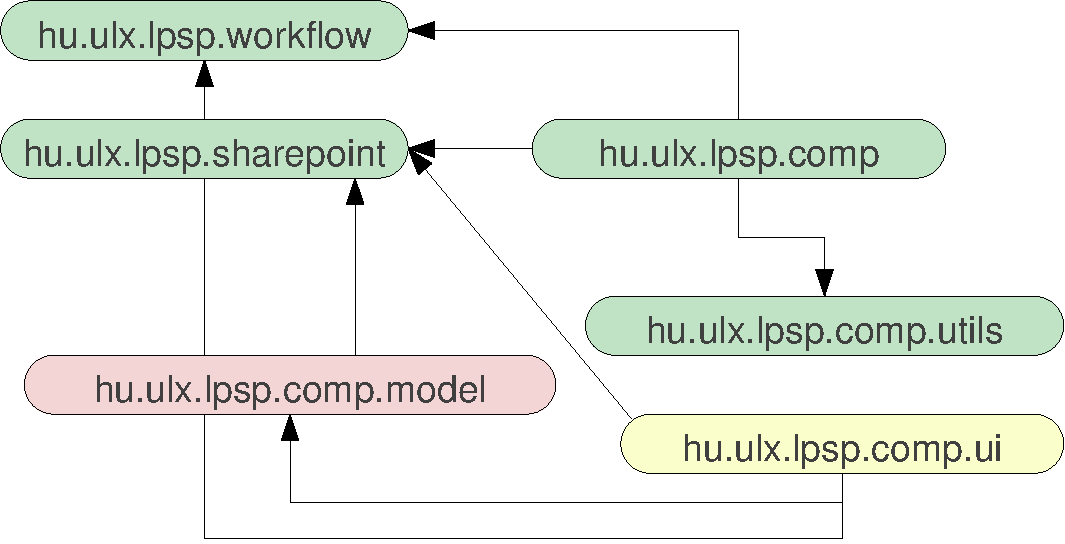
\includegraphics[width=425px,keepaspectratio]{design-packages-wf.pdf}
\caption{Packages of the workflow-enabled SharePoint extension}
\label{fig:design-packages-wf}
\end{figure}

\autoref{fig:design-packages-wf} shows the updated UML package diagram of our
solution. The recently introduced \textbf{\emph{hu.ulx.lpsp.workflow}} package can be divided to three
parts:

\begin{itemize}
\item controller classes
\item entity classes
\item parser classes
\end{itemize}

\subsubsection*{Controller classes}

Given that jBPM provides a REST API to control the workflow engine, the client
library can be quite simple. Its business logic is implemented in a single
class, called \emph{WFHandler}. It should provide the following features:

\begin{itemize}
\item authentication handling
\item wrappers for used REST method calls
\item mapping between JSON data and entity classes
\item parsing task data from HTML forms
\end{itemize}

Note that jBPM itself is stateless, but the client library mimics a stateful
connection to avoid asking for connection parameters before all operations.

A decision we made here is that we don't support all kind of process
definitions, only the document-based ones. Our definition of being
document-based is:

\begin{itemize}
\item the process definition has a string variable named \emph{url}
\item the process definition has a task form, where this URL can be specified on process start
\end{itemize}

\subsubsection*{Parser classes}

Whenever a REST method call returns from jBPM, the result can one of the following formats:

\begin{itemize}
\item HTML, when getting a task form
\item XML, when asked for process instance data
\item JSON, in any other case
\end{itemize}

There are multiple problems with arbitrary HTML in our case:

\begin{itemize}
\item jBPM expects an embedded HTML engine in the client, which is not the case with our SWING-based Java user interface
\item once the form is submitted, the server would instruct the user to close
the window, which would be inconsistent with our ``the window is
closed when no more input should be provided'' approach
\item in our case the form should be extended to ask for document-management details as well
\end{itemize}

When using HTML, there are several ways to express business decision. Some example:

\begin{itemize}
\item using separate buttons for each decision
\item using the HTML \texttt{<select>} tag to list choices
\item using radio buttons
\item some AJAX method
\end{itemize}

It is obviously impossible to support all these methods, so we declared a
second constraint here: decisions should be described using submit buttons.

As a result, the \emph{FormParser} class can simply parse submit tag name-value
pairs from the form to detect multiple choices, and the list of values is sent
to the user interface.

\subsubsection*{Entity classes}

Whenever a JSON data structure is returned by a REST method call, the client
library provides the results as an entity class. A convention we follow here is that every type has two entity classes:

\begin{itemize}
\item \emph{TypeRef}: a reference to the instance of the given type itself
\item \emph{TypeRefWrapper}: a class for the collection of instance references of the given type
\end{itemize}

This is handy because this way we don't have to decide what Java interface
(\emph{java.util.List} could be a candidate) can cover all the details the
server provides about an instance list.

The following types are handled by the client:

\begin{itemize}
\item \emph{Process}: is a process definition
\item \emph{ProcessInstance}: is a process instance
\item \emph{NodeInstance}: is a node instance
\item \emph{Task}: a task instance
\end{itemize}

The type names are in sync with the REST API, which is more helpful than simply
trying to be consistent with ourselves -- and store the result of a task query
in a task instance type.

\subsection{jBPM and the BPM console server}

The only functionality we need, but is not provided by the BPM console server
REST API is the audit log. jBPM itself logs all the necessary information in
its SQL backend, so we need the following steps to export this knowledge to the
REST API:

\begin{itemize}
\item extend the interface of the integration layer in the BPM console server
\item implement the extended interface in jBPM
\item extend the REST API to use the extended interface
\end{itemize}

Given that jBPM and the BPM console are separate project, first we need an
implementation in jBPM, then the new methods can be added to the integration
layer interface in the BPM console.

\subsubsection*{Extending jBPM}

We need three new features -- the ability to get information about:

\begin{itemize}
\item historic process instances
\item node instances of a process instance
\item task instances of a process instance
\end{itemize}

In case of historic process instances, the following steps are needed:

\hyphenation{Process-Instance-Db-Log}

\begin{itemize}
\item a new \emph{getHistoricProcessInstances} method is introduced in the \emph{ProcessManagement} interface implementation, calling
\item a new \emph{getInactiveProcessInstanceLogsByProcessId} method, to be introduced in the \emph{CommandDelegate} class of the integration implementation package, calling
\item a new \emph{findInactiveProcessInstances} method, to be introduced in the \emph{ProcessInstanceDbLog} class in the audit package of jBPM
\end{itemize}

This last method uses Hibernate to get the necessary information from the SQL
database. The naming of the new methods is chosen to be consistent with the
existing API.

Once the process instances are accessible, we need node instances. The
following new methods are introduced to achieve this:

\begin{itemize}
\item a new \emph{getNodeInstances} method in the \emph{ProcessManagement} interface implementation, calling
\item a new \emph{getNodeInstanceLogsByProcessInstanceId} method, to be introduced in the \emph{CommandDelegate} class
\end{itemize}

Modification of the \emph{ProcessInstanceDbLog} class is not necessary, support
for querying node instances is already implemented there. However, the
\emph{ProcessManagement} interface implementation should turn the Java object
to a JSON serialization, which is handled by a new \emph{nodeInstance()} method
in the \emph{Transform} class of the integration implementation package.

\begin{figure}[p]
\centering
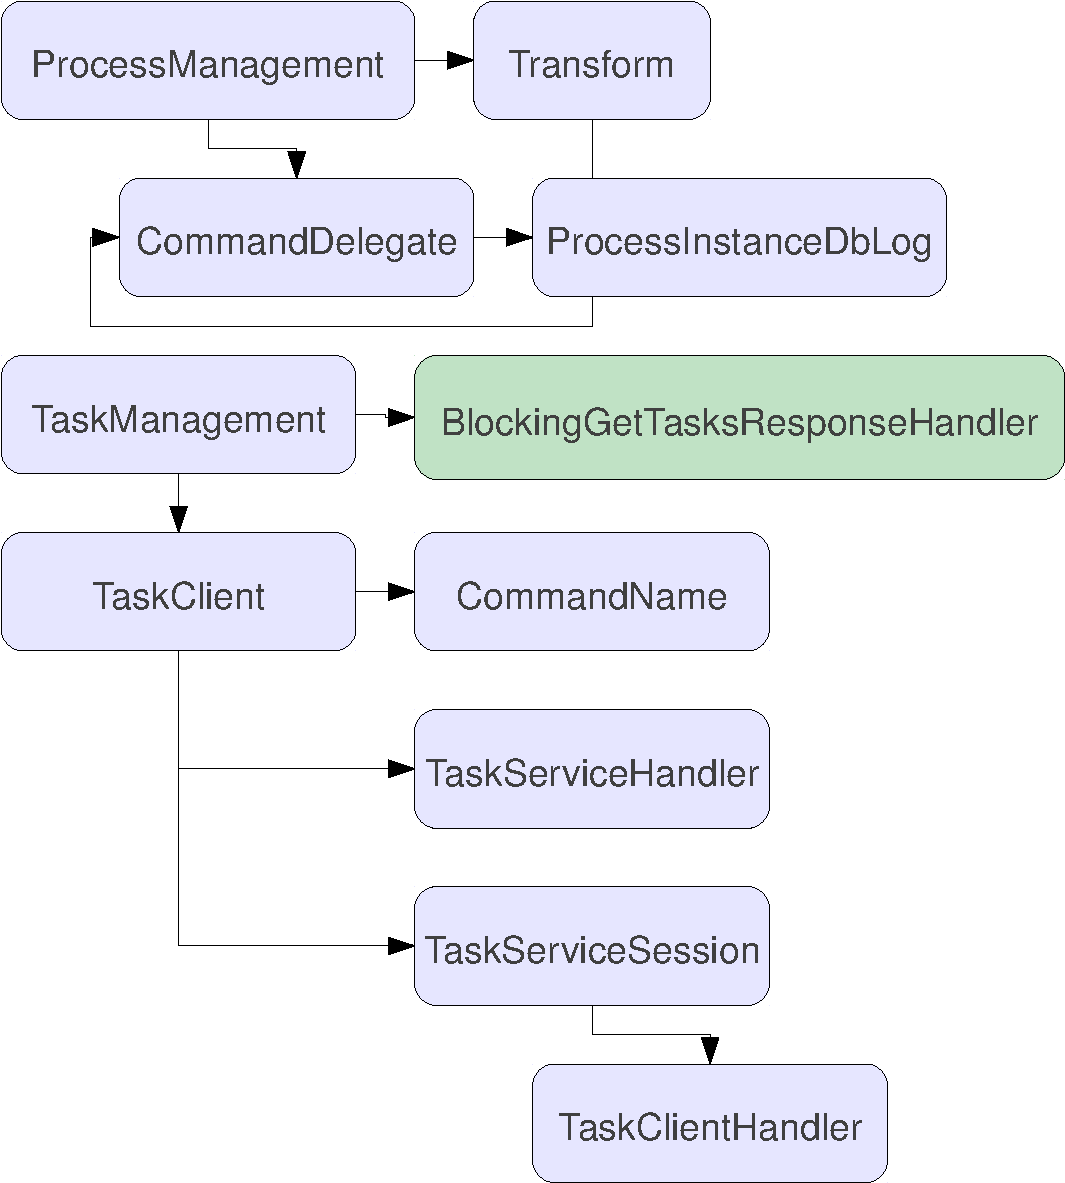
\includegraphics[width=300px,keepaspectratio]{jbpm-modified-classes.pdf}
\caption{Audit log provider classes of jBPM. Blue classes are modified, the green class is a new one.}
\label{fig:jbpm-modified-classes}
\end{figure}

Finally, getting information about task instances of a process instance is a
bit more complex. The following changes are introduced:

\begin{itemize}
\item A new \emph{getProcessInstanceTasks} method in the \emph{TaskManagement}
	interface implementation. This will instantiate a new
	\emph{BlockingGetTasksResponseHandler} class, implementing a new
	\emph{GetTasksResponseHandler} interface. Then it will call:
\item A new \emph{getTasksByProcessInstanceId} method in the \emph{TaskClient} class. This will use two new constants (one is \emph{QueryTasksByProcessInstanceId}, the other is \emph{QueryTasksByProcessInstanceIdResponse}), provided by the \emph{CommandName} class. This new method will call:
\item the \emph{TaskServerHandler} class, which should be extended to handle the \emph{QueryTasksByProcessInstanceId} token, which will call:
\item A new \emph{getTasksByProcessInstanceId} method in the \emph{TaskServiceSession} class. This will invoke a new stored procedure, named \emph{TasksByProcessInstanceId}. Finally it will call:
\item the \emph{TaskClientHandler} class, handling the \emph{QueryTasksByProcessInstanceIdResponse} token, calling back the original \emph{BlockingGetTasksResponseHandler} implementation.
\end{itemize}

The interaction between these classes can be seen on \autoref{fig:jbpm-modified-classes}.

\subsubsection*{Extending the BPM console server}

Once the implementation of the integration layer in jBPM is in place, we can
export these features in the REST API, using the following paths:

\begin{itemize}
\item \url{process/definition/history/{id}/instances}: process instances
\item \url{process/history/{processInstanceId}/nodes}: node instances
\item \url{tasks/history/{processInstanceId}}: task instances
\end{itemize}

When a query about a process instance is received, then:

\begin{itemize}
\item A new \emph{getCompletedInstances} method in the \emph{ProcessMgmtFacade} class is invoked, calling:
\item The new \emph{getHistoricProcessInstances} method in the \emph{ProcessManagement} interface of the integration layer.
\end{itemize}

Similarly, if a query about a node instance is received, then:

\begin{itemize}
\item A new \emph{getCompletedNodes} method in the same \emph{ProcessMgmtFacade} class is invoked, calling:
\item The new \emph{getNodeInstances} method in the above \emph{ProcessManagement} interface.
\end{itemize}

In this case serialization to JSON has to be handled by the new
\emph{NodeInstanceRef} and \emph{NodeInstanceRefWrapper} classes. Note that
these private classes are independent from the ones having the same name in the
client library, as only the JSON output is public, allowing loose coupling.

Finally, once a query about a task is received, then:

\begin{itemize}
\item A new \emph{getTasksForProcessInstance} method in the \emph{TaskListFacade} class is invoked, calling:
\item The new \emph{getProcessInstanceTasks} method in the \emph{TaskManagement} interface of the integration layer.
\end{itemize}

\subsection{User interface}

Workflow support affects the user interface in the following areas:

\begin{itemize}
\item menu items
\item BASIC macros
\item UNO interfaces and services
\item Java Implementation classes
\item Dialog classes
\end{itemize}

The rest of this chapter details these modifications.

\subsubsection*{Menu items}

The following new menu items are introduced for workflow integration:

\begin{itemize}
\item \emph{Start workflow}: starts a new process instance associated with the current document.
\item \emph{Workflow audit log}: shows a window with information about historic process instances.
\end{itemize}

\subsubsection*{BASIC macros}

These menu items call the following BASIC macros in the \emph{LPSP.menu} script library:

\begin{itemize}
\item \emph{openWorkflow()} is called when the workflow definition list is opened.
\item \emph{workflowProcesses()} is called when the process instance list is shown.
\end{itemize}

\subsubsection*{UNO interfaces and services}

To allow the macros to invoke Java methods, first we need a UNO specification.
Two new interfaces are introduced:

\begin{itemize}
\item \emph{XJbpmWorkflow}: invoke the Java library to start a new process instance.
\item \emph{XJbpmWorkflowProcesses}: invoke the Java library to show historic process instances.
\end{itemize}

Given that it's not possible to instantiate interfaces, new services are
defined to implement these interfaces:

\begin{itemize}
\item \emph{JbpmWorkflow}: implements \emph{XJbpmWorkflow}
\item \emph{JbpmWorkflowProcesses}: implements \emph{XJbpmWorkflowProcesses}
\end{itemize}

With this, the basic macros can call the following UNO services:

\begin{itemize}
\item Start workflow: calls \emph{JbpmWorkflow::execute()}.
\item Workflow audit log: calls \emph{JbpmWorkflowProcesses::execute()}.
\end{itemize}

\subsubsection*{Java implementation classes}

The UNO services invoke the following methods in the Java implementation:

\begin{itemize}
\item Start workflow: \emph{JbpmWorkflowImpl.execute()}
\item Workflow audit log: \emph{JbpmWorkflowProcessesImpl.execute()}
\end{itemize}

\subsubsection*{Dialog classes}

\autoref{fig:design-wfui} shows the new dialog classes used by the workflow
UNO service implementations.

\begin{figure}[p]
\centering
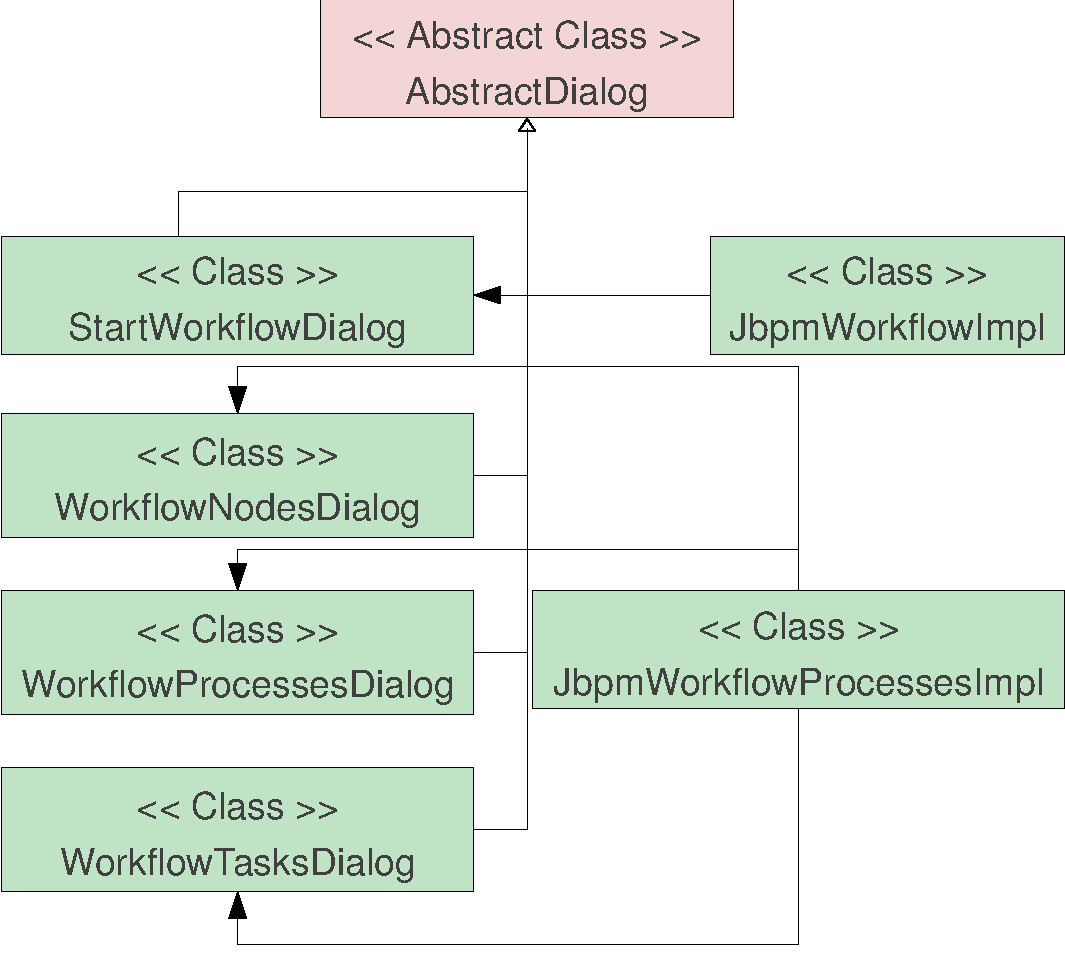
\includegraphics[width=400px,keepaspectratio]{design-wfui.pdf}
\caption{Classes of the workflow user interface}
\label{fig:design-wfui}
\end{figure}

To start a new workflow, a single new dialog -- \emph{StartWorkflowDialog} --
is planned, that will show a list of process definitions available.

The audit log will have three new dialogs:

\begin{itemize}
\item \emph{WorkflowProcessesDialog} is the initial window, showing the process instance list.
\item \emph{WorkflowNodesDialog} can show node instances of a process instance, opened from the process instance list.
\item \emph{WorkflowTasksDialog} displays task instances of a process instance, similarly opened by the process instance dialog.
\end{itemize}

Additionally here and there existing dialogs have to be extended with
workflow-specific items:

\begin{itemize}
\item \emph{CommentVersionDialog}: When saving, new controls are needed to control decisions and completing of workflow tasks.
\item \emph{FilePickerDialog}: During open, the file picker has to be improved to allow task claiming/releasing, also task listing should be handled here.
\item \emph{ConfigServerDialog}: The table showing properties of different connections should show workflow server URL.
\item \emph{ServerDialog}: New controls are needed to be able to edit workflow URL of a server connection.
\end{itemize}

All modifications in the existing dialog classes should tolerate the lack of a
workflow server, so document management integration can be used as a standalone
feature as well.
